\documentclass{article}
\usepackage[T1]{fontenc}
\usepackage{lmodern}
\usepackage{graphicx}
\usepackage{amsmath,amssymb}
\usepackage[a4paper,margin=2cm]{geometry}
\usepackage[absolute,overlay]{textpos}
\setlength{\TPHorizModule}{1mm}
\setlength{\TPVertModule}{1mm}
\usepackage[indonesian]{babel}
\usepackage{hyperref}
\setlength{\emergencystretch}{2em}
% unit: Halaman 42

\begin{document}

% === Halaman 42 (llm) ===

\vspace{50mm}

The \href{https://www.eff.org}{EFF}'s US\$250,000 \href{https://en.wikipedia.org/wiki/DEScracker}{DES cracking machine} contained 1,856 custom chips and could brute force a DES key in a matter of days -- the photo shows a DES Cracker circuit board fitted with several Deep Crack chips (Sumber Wikipedia).

% deskripsi: Foto papan sirkuit DES Cracker yang dilengkapi dengan beberapa chip Deep Crack.
% bbox normalisasi: [0.3350, 0.1360, 0.6210, 0.6630]
\begin{textblock*}{60.06mm}(70.35mm,40.39mm)
\noindent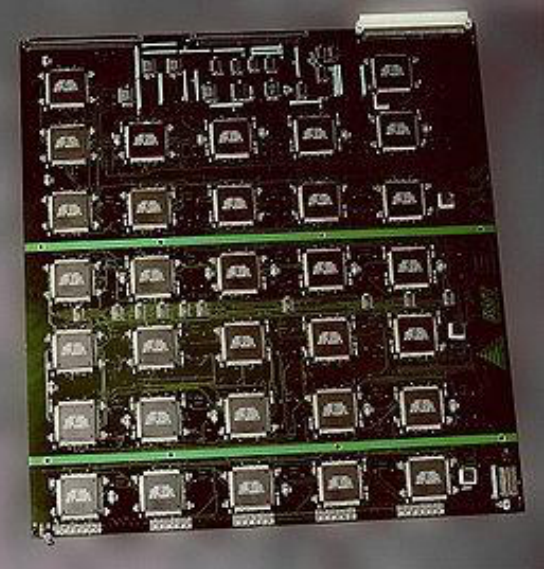
\includegraphics[width=60.06mm,height=156.52mm]{../../images/llm/page_042_img_01.png}%
\end{textblock*}

\end{document}
